This is not the full 2020 exam, only the first two exercises. 

%-----------------------
\subsection*{Exercise 1}
Let us consider a spherically symmetric body of radius $R$.

\begin{enumerate}
\item (1 pt) use symmetry considerations with regards to the 3 axis
to arrive at the moment of inertia $I$:
\begin{equation}
I=\frac{8\pi}{3} \int_0^R \rho(r) r^4 dr 
\end{equation}
\item (1/2 pt) The density inside the sphere is given by
\[
\rho(r)=\rho_0 \left[ a \left(\frac{r}{R}\right)^2+ b \left(\frac{r}{R}\right) + c \right]
\]
Compute coefficients $a,b,c$ such that the density matches the curve on the following figure:

\begin{center}
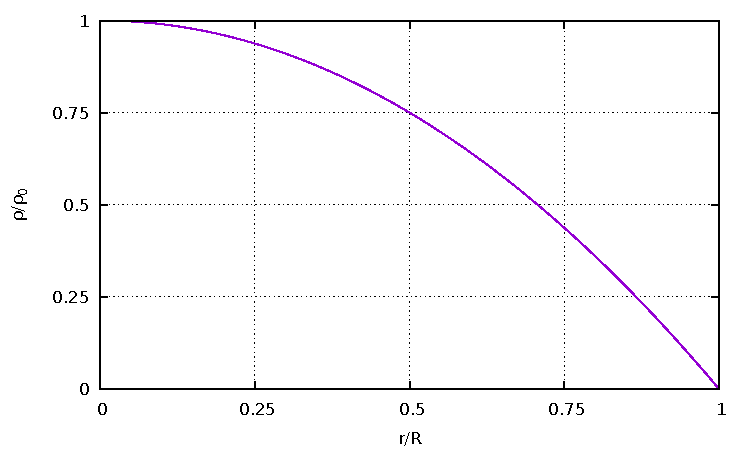
\includegraphics[width=9cm]{images/gravity/exam2020/rho.pdf}
\end{center}

\item (1 pt) Compute the total mass $M$ of the planet using this expression for the density.
\item (1 pt) Compute the moment of inertia $I$
\item (1/2 pt) Can $I$ be written $I=fMR^2$? if so, give $f$.
\item (1/2 pt) What are the dimensions of $\rho$, $I$ and $M$?
\end{enumerate}

\subsection*{Exercise 1 - answer}

Question 1 was treated in class.  
Looking at the figure, we see that $\rho(r=0)=\rho_0$, i.e. $c=1$.
Also, we see that $\rho(r=R)=0$, i.e.
\[
\rho_0 \left[ a +b + 1 \right] =0 
\]
or, $a+b=-1$.
Finally, we see that $\rho(r=R/2)=3\rho_0/4$, so
\[
\rho_0 \left[ \frac{a}{4} +\frac{b}{2} +1 \right] = \frac{3}{4}\rho_0
\]
or, $a/4 + b/2 = -1/4$.
This leads to $a=-1$ and $b=0$ so 
\[
\rho(r) = \rho_0 \left[ 1 - \left(\frac{r}{R}\right)^2  \right]
\]

The total mass is given by 
\begin{eqnarray}
M 
&=& \int_V \rho(r) dV \nn\\
&=&  4\pi \int_0^R  \rho(r) r^2 dr \nn\\
&=&  4\pi \int_0^R   \rho_0 \left[ 1 - \left(\frac{r}{R}\right)^2  \right]  r^2 dr \nn\\
&=&  4\pi \rho_0  \int_0^R   \left[ r^2 - \frac{r^4}{R^2}  \right]  dr \nn\\
&=& \frac{8 \pi}{15} \rho_0 R^3
\end{eqnarray}

The moment of inertia $I$ is 
\begin{eqnarray}
I 
&=&  \frac{8\pi}{3} \int_0^R  \rho(r) r^4 dr \nn\\
&=& \frac{16 \pi}{105} \rho_0 R^5
\end{eqnarray}

Finally, 
\[
I = \frac{16 \pi}{105} \rho_0 R^5 = \frac{2}{7} (\frac{8 \pi}{15} \rho_0 R^3) R^2
\]
so $f=2/7$.


%-----------------------
\subsection*{Exercise 2}

Let us consider the same sphere as in the previous exercise, and the same density profile $\rho(r)$.
The gravitational potential satisfies the Poisson equation:
\begin{equation}
\Delta U = 4 \pi {\cal G} \rho({\vec r}) \label{exam2020:eqlap}
\end{equation}
and we have the following relationship between the gravitational acceleration 
vector and the potential: ${\vec g}=-{\vec \nabla} U$.

\begin{enumerate}
\item (1/2 pt) Write explicitely Eq.(\ref{exam2020:eqlap}) for a point inside the sphere and a point outside the sphere.
\item (1 pt) Compute $g(r)$ and $U(r)$ for a point inside the sphere as a function of $r$. Use 
$\lim_{r\rightarrow 0} g(r) \neq \infty$
to get rid of an integration constant.
\item (1 pt) Compute $g(r)$ and $U(r)$ for a point outside the sphere as a function of $r$. 
Use $\lim_{r\rightarrow\infty}U(r)=0$ to get rid of another integraion constant.
\item (1 pt) Use the continuity of $g(r)$ and $U(r)$ at $r=R$ 
to compute the last two remaining integration constants.
\end{enumerate}

%-----------------------
\subsection*{Exercise 2 - answer}

Inside the sphere Eq.(\ref{exam2020:eqlap}) is

\begin{equation}
\frac{1}{r^2} \frac{\partial}{\partial r} \left( r^2 \frac{\partial U}{\partial r} \right) = 4 \pi {\cal G} 
\rho_0 \left[ a \left(\frac{r}{R}\right)^2+ b \left(\frac{r}{R}\right) + c \right]  \nn
\end{equation}

We could use the values of $a$, $b$ and $c$ obtained above but I here choose not to, in order to show that 
this exercise can be carried out independently from the first one. Then: 

\begin{equation}
\frac{\partial}{\partial r} \left( r^2 \frac{\partial U}{\partial r} \right) = 4 \pi {\cal G} 
\rho_0 \left[ a \frac{r^4}{R^2}+ b \frac{r^3}{R} + c r^2 \right] \nn
\end{equation}

\begin{equation}
r^2 \frac{\partial U}{\partial r} = 4 \pi {\cal G} \rho_0 \left[ a \frac{r^5}{5R^2}+ b \frac{r^4}{4R} + c \frac{r^3}{3} \right] + A  \nn
\end{equation}

\begin{equation}
\frac{\partial U}{\partial r} = 4 \pi {\cal G} \rho_0 \left[ a \frac{r^3}{5R^2}+ b \frac{r^2}{4R} + c \frac{r}{3} \right] + \frac{A}{r^2} \nn
\end{equation}
so that 
\begin{equation}
g(r)=-\frac{\partial U}{\partial r} = -4 \pi {\cal G} \rho_0 \left[ a \frac{r^3}{5R^2}+ b \frac{r^2}{4R} + c \frac{r}{3} \right] + \frac{A}{r^2} \nn
\end{equation}
We use $\lim_{r\rightarrow 0} g(r) \neq \infty$ to arrive at $A=0$.
Finally 

\begin{equation}
U_{in}(r) = 4 \pi {\cal G} \rho_0 \left[ a \frac{r^4}{20R^2}+ b \frac{r^3}{12R} + c \frac{r^2}{6} \right] + B \nn
\end{equation}

With $a=-1$, $b=0$ and $c=1$:
\begin{eqnarray}
g_{in}(r) &=&  -4 \pi {\cal G} \rho_0 \left[ - \frac{r^3}{5R^2}+   \frac{r}{3} \right]  \nn\\
U_{in}(r) &=& 4 \pi {\cal G} \rho_0 \left[ - \frac{r^4}{20R^2} +  \frac{r^2}{6} \right] + B  \nn
\end{eqnarray}

Outside the sphere we must solve 
\begin{equation}
\frac{1}{r^2} \frac{\partial}{\partial r} \left( r^2 \frac{\partial U}{\partial r} \right) = 0 \nn
\end{equation}

\begin{equation}
r^2 \frac{\partial U}{\partial r}  = C \nn 
\end{equation}
\begin{equation}
\frac{\partial U}{\partial r}  = \frac{C}{r^2} \nn
\end{equation}
\begin{equation}
U_{out}(r) = -\frac{C}{r} + D  \nn
\end{equation}
We use $\lim_{r\rightarrow\infty}U(r)=0$ to arrive at $D=0$ so that 
\begin{eqnarray}
g_{out}(r) &=& -\frac{C}{r^2}  \nn\\
U_{out}(r) &=& -\frac{C}{r} \nn
\end{eqnarray}

Both fields should match at $r=R$:
\begin{eqnarray}
g_{in}(r=R) &=& g_{out}(r=R) \nn\\
U_{in}(r=R) &=& U_{out}(r=R) \nn
\end{eqnarray}
i.e.
\[
-4 \pi {\cal G} \rho_0 \left[ a \frac{R^3}{5R^2}+ b \frac{R^2}{4R} + c \frac{R}{3} \right]  =   -\frac{C}{R^2} 
\]
so 
\[
C = 4 \pi {\cal G} \rho_0 R^3 \left[ \frac{a}{5}+ \frac{b}{4} +  \frac{c}{3} \right]   
\]
Now, 
\[
4 \pi {\cal G} \rho_0 \left[ a \frac{R^4}{20R^2}+ b \frac{R^3}{12R} + c \frac{R^2}{6} \right] + B = -\frac{C}{R} 
\]
\[
4 \pi {\cal G} \rho_0 R^3 \left[  \frac{a}{20}+ \frac{b}{12} +  \frac{c}{6} \right] + B R = -4 \pi {\cal G} \rho_0 R^3 \left[  \frac{a}{5}+  \frac{b}{4} +  \frac{c}{3} \right]   
\]
so 
\[
B R= -4 \pi {\cal G} \rho_0 R^3 \left[
 \frac{a}{5}+ \frac{a}{20}
+\frac{b}{4}+ \frac{b}{12}
+\frac{c}{3}+ \frac{c}{6}
\right]
\]
\[
B = -4 \pi {\cal G} \rho_0 R^2 \left[
 \frac{a}{4}
+\frac{b}{3}
+\frac{c}{2}
\right]
\]

With $a=-1$, $b=0$ and $c=1$:
\[
B = - \pi {\cal G} \rho_0 R^2  
\qquad
C = \frac{8\pi}{15} {\cal G} \rho_0 R^3 
\]

Finally

\begin{eqnarray}
g_{in}(r) &=&  -4 \pi {\cal G} \rho_0 \left[ - \frac{r^3}{5R^2}+   \frac{r}{3} \right] \nn \\
U_{in}(r) &=& 4 \pi {\cal G} \rho_0 \left[ - \frac{r^4}{20R^2} +  \frac{r^2}{6} \right] 
 - \pi {\cal G} \rho_0 R^2  \nn\\
g_{out}(r) &=& - \frac{8\pi}{15} {\cal G} \rho_0 R^3 \frac{1}{r^2} \nn\\ 
U_{out}(r) &=& -\frac{8\pi}{15} {\cal G} \rho_0 R^3 \frac{1}{r}  \nn
\end{eqnarray}

Also, remembering that the mass of the planet is  $M=\frac{8 \pi}{15} \rho_0 R^3$
so that 
\begin{eqnarray}
g_{out}(r) &=& - \frac{ {\cal G} M}{r^2} \nn\\ 
U_{out}(r) &=& -  \frac{ {\cal G} M}{r} \nn 
\end{eqnarray}
No surprise there...



